\begin{figure}[t]
\centering
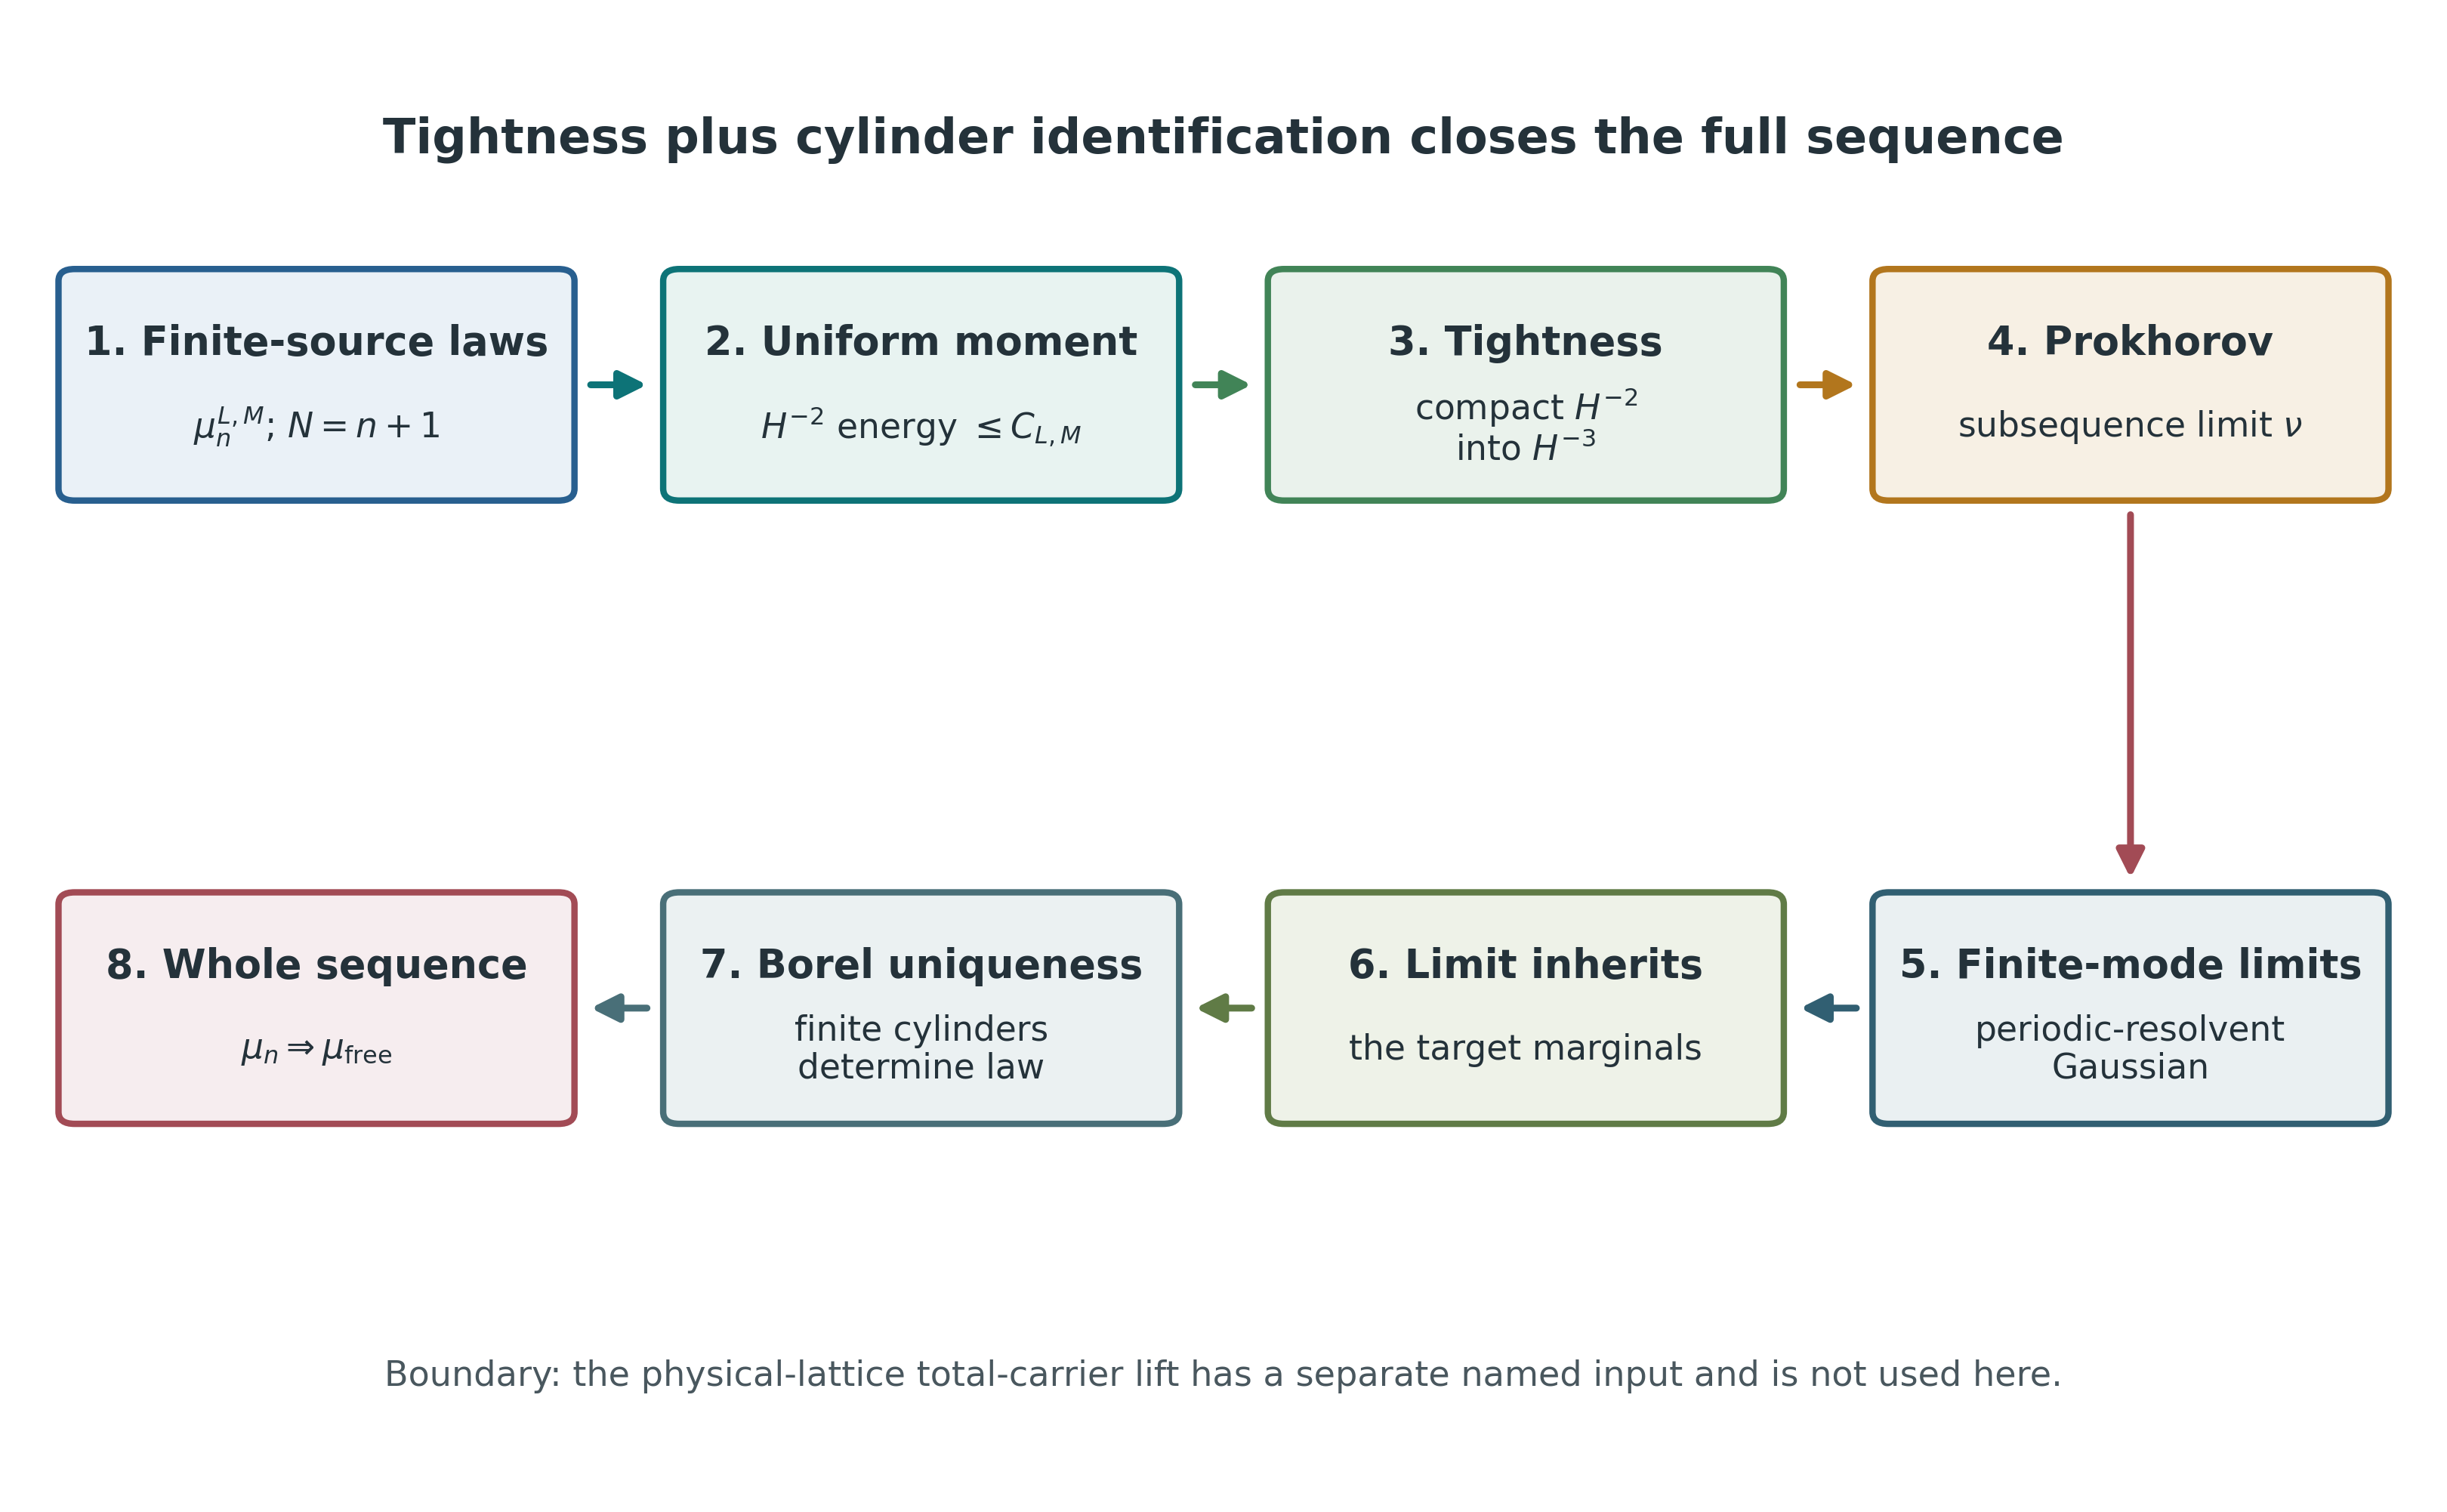
\includegraphics[width=\linewidth]{figures/weak_limit_spine.png}
\caption{The spine of the limit argument. The first box is the point of departure, the finite-source lattice laws; the seven after it carry the argument: the uniform $H^{-2}$ moment; tightness on the carrier; Prokhorov extraction of a subsequential limit; the finite-mode limits from the marginal computations; the limit inherits the target marginals; cylinder-to-Borel uniqueness identifies that limit; and whole-sequence convergence closes it. The last step is the whole-sequence conclusion, not merely a subsequential one. Two inputs are not drawn, because they are settled before this half begins: the carrier construction (move~2 of \cref{sec:intro}) and the covariance limit (part of move~1), which is where the target covariance comes from. Two reading notes. The figure's own footer annotation calls the total-carrier lift a separate input that is not used here; that annotation records the development's implementation choice and is superseded by \cref{lem:lift-representative} and \cref{rem:lift-development}, which prove the paper's lift total and Borel outright. And the figure labels the mass $M$ where the text writes $m$; the index $n$ is the text's own mesh index, not the text's $N$.}
\label{fig:spine}
\end{figure}
